\documentclass[a4paper]{article}

\usepackage[T1]{fontenc}
\usepackage[spanish]{babel}

\usepackage{graphicx, geometry, array, booktabs, float, hyperref, setspace}
\usepackage[dvipsnames]{xcolor}

\hypersetup{
    colorlinks=true,
    linkcolor=black,
    urlcolor=RoyalBlue,
}


\begin{document}

\begin{titlepage}
    \newgeometry{top=0.6in,bottom=0.6in,right=1in,left=1in}

    \centering
    \hfill
    \begin{minipage}{0.7\textwidth}
            \centering
            \LARGE
            \textsc{\textbf{Facultad de Ingeniería}}\\[0.1cm]
            \textsc{\textbf{Universidad de Buenos Aires}}
        \end{minipage}%
        \begin{minipage}{2.6cm}
            \centering
            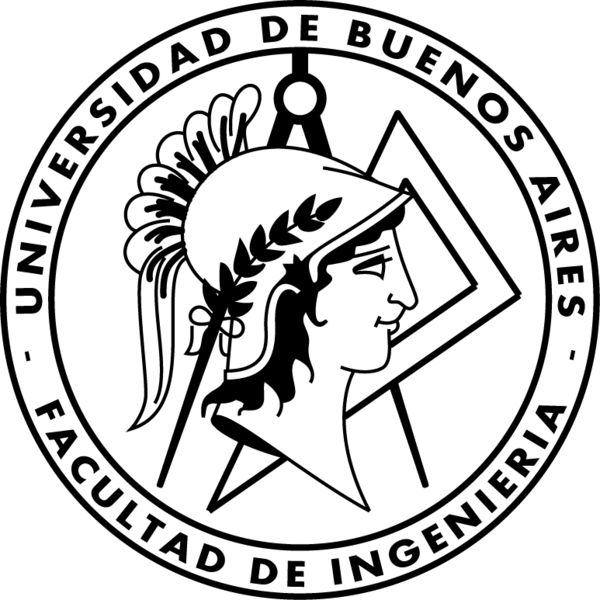
\includegraphics[width=2.6cm]{./img/fiuba.png}
        \end{minipage}

    \vspace{3cm}
    \huge \bfseries Propuesta de Trabajo Profesional \\
    \LARGE \bfseries Licenciatura en Análisis de Sistemas, Ingeniería en Informática
    \vspace{2cm}

    \rule{\linewidth}{0.3mm} \\[0.1cm]
    \huge \bfseries Sistema de detección en tiempo real de publicidad en la vía pública \\
    \rule{\linewidth}{0.3mm}\\[0.7cm]

    \large \emph{Tutor:} Ing. Martín Buchwald\\[0.6cm]
    \begin{minipage}{0.4\textwidth}
        \begin{flushleft}
            \centering
            \large del Mazo, Federico \\
            100029
        \end{flushleft}
    \end{minipage}
    \begin{minipage}{0.4\textwidth}
        \begin{flushright}
            \centering
            \large Pastine, Casimiro \\
            100017
        \end{flushright}
    \end{minipage}

\end{titlepage}

\restoregeometry
\tableofcontents
\newpage

\section{Motivación}
Dentro del marco de trabajo profesional de las carreras de Licenciatura en Análisis de Sistemas y de Ingeniería en Informática de la Facultad de Ingeniería, Universidad de Buenos Aires, se presenta la siguiente propuesta de proyecto con el objetivo de desarrollar un sistema de detección de publicidades en la vía pública en tiempo real.

El interés detrás de este proyecto radica en la creciente intrusión e invasión de publicidades no deseadas en nuestro entorno cotidiano. Este proyecto busca concientizar y ofrecer una solución práctica a esta problemática, enfocándose principalmente en la detección, y luego permitiendo al usuario aplicar un post-procesamiento configurable para difuminar, resaltar o transformar de otra manera lo detectado.

\section{Objetivos}
\begin{itemize}
    \item Aplicar los conocimientos interdisciplinarios de comprensión y evaluación de sistemas aprendidos en nuestra carrera académica en un campo enteramente nuevo para nosotros como lo es \emph{Computer Vision}.
    \item Realizar un proyecto integral con su debida investigación y comprensión del estado del arte en las disciplinas relevantes, abarcando desde el entrenamiento de un modelo de clasificación de objetos hasta el despliegue del sistema en algún entorno fácilmente accesible por el usuario final.
    \item Encontrarnos con desafíos prácticos como la falta de los datos necesarios para el modelo a entrenar y la evaluación y comparación de distintos métodos para lograr un rendimiento aceptable y encontrar las soluciones adecuadas para los obstáculos que vayan apareciendo, sopesando las distintas alternativas posibles que surgirán durante el desarrollo del trabajo.
    \item Lograr hacer un sistema de código abierto, modularizable y extensible tal que en un futuro se pueda cambiar cualquier eslabón de su cadena como los objetos a detectar, el algoritmo de detección y rastreo de objetos o el post procesamiento a aplicar.
\end{itemize}

\section{Descripción del problema}
\subsection{Computer Vision}
El campo de \emph{Computer Vision} se refiere a la disciplina de la inteligencia artificial que se ocupa de permitir a las computadoras ``ver'' y comprender el mundo visual de la misma manera que lo hacen los seres humanos. Utiliza diversas técnicas y algoritmos para adquirir, procesar, analizar y comprender imágenes y videos digitales con el objetivo de extraer información significativa y tomar decisiones basadas en ella.

En los últimos años este campo ha experimentado un crecimiento y una atención considerable debido al aumento del poder computacional, la disponibilidad de grandes conjuntos de datos y los avances en el aprendizaje automático y las redes neuronales.

Uno de los avances más revolucionarios dentro del campo de \emph{Computer Vision} es el uso de las \emph{Redes Neuronales Convolucionales (CNN)}. Son un tipo de arquitectura de redes neuronales especialmente diseñadas para el procesamiento de datos de imágenes o señales de audio. La característica determinante es la capa convolucional de la red, a través de la cual las CNN aprenden a extraer características y combinan esta información para realizar tareas de clasificación y reconocimiento de patrones.

Uno de los problemas iniciales de \emph{Computer Vision} es la clasificación de imágenes: Partiendo de una imagen, queremos saber si la misma contiene un objeto deseado. Por ejemplo, podríamos tener una foto en la vía pública y querer saber si contiene o no a un cartel publicitario.

\begin{figure}[H]
    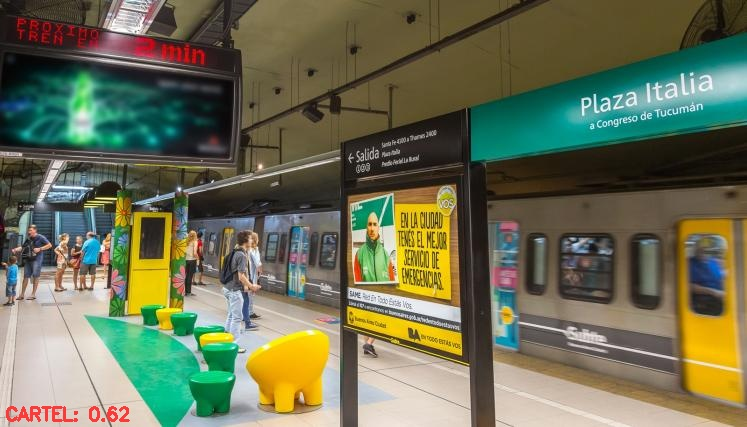
\includegraphics[width=0.7\textwidth]{./img/classif.jpg}
    \centering
\end{figure}

El paso siguiente a esto es la detección de objetos. Ya no solo importa si el cartel publicitario está presente, sino exactamente en qué porción de la imagen lo está.

\begin{figure}[H]
    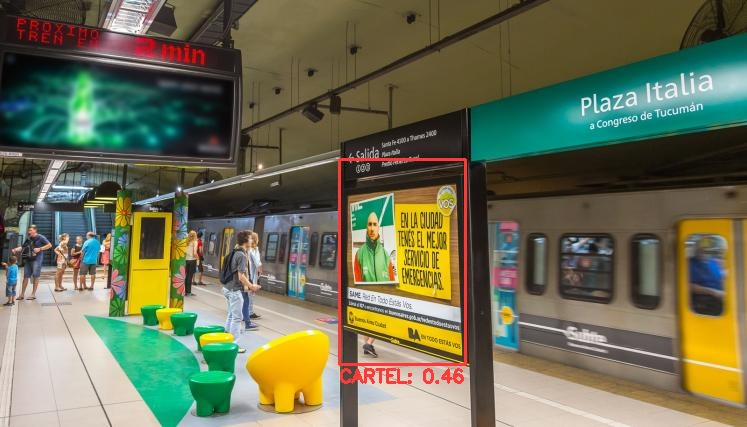
\includegraphics[width=0.7\textwidth]{./img/detection.jpg}
    \centering
\end{figure}

Naturalmente el paso siguiente a detectar objetos en imágenes estáticas (fotografías), es hacerlo en video. Queremos detectar cuándo un objeto entra en escena, cuando sale, y poder seguirle el rastro en todo momento. Esto se denomina \emph{Object Tracking} y es la técnica principal sobre la cual basamos nuestro trabajo.

El paso final en cuanto a la detección de objetos en nuestro trabajo incluye la meta de hacerlo en tiempo real. A diferencia de analizar un video pregrabado, donde es prescindible la velocidad de procesamiento, esto plantea el desafío considerable de tener que procesar los cuadros del video más rápido de lo que están siendo capturados para poder mostrar el resultado final inmediatamente.

\subsection{Despliegue}
En el despliegue del sistema se nos presentan alternativas que van a ser evaluadas en términos del rendimiento y la experiencia de usuario que buscamos alcanzar.

El mínimo entregable que proponemos para nuestro trabajo es una herramienta de procesamiento de video pregrabado que se corra localmente por línea de comando y devuelva un video procesado como salida.

Nuestra meta principal es entregar una experiencia de usuario con una interfaz mejor a la de línea de comando, que pueda ser utilizada desde cualquier parte, sin requerir ningún tipo de instalación previa. Por esto es que consideramos que la interfaz ideal del sistema es en un sitio web.
El hecho de que la interfaz sea una página web nos da dos posibles arquitecturas a evaluar. Por un lado contemplamos la arquitectura cliente/servidor, mientras que su contraposición natural es un sistema que sea ejecutado solamente en el cliente local.

En una arquitectura cliente/servidor, la capacidad computacional del cliente no es relevante, pero la complejidad principal del sistema recae en poder minimizar la latencia entre el cliente y el servidor. Por otro lado, en una arquitectura sin servidor donde todo se ejecuta localmente, el principal desafío es poder seguir ofreciendo una buena experiencia de usuario independientemente del poder computacional del dispositivo sobre el cual corre el sistema. Sobre esta última idea, una alternativa disponible es la de utilizar \emph{WebAssembly}, ya que nos permitiría desarrollar el sistema en cualquier lenguaje de programación, donde podamos enfocarnos en la velocidad de procesamiento por sobre lo disponible en el entorno web.

\subsection{Tecnologías Relevantes al Trabajo}
El lenguaje de programación que vamos a utilizar para realizar el trabajo es \emph{Python}, debido a que es ampliamente utilizado en el campo de \emph{Computer Vision} gracias a su flexibilidad, bibliotecas especializadas y facilidad de uso.

La principal herramienta que utilizaremos es \emph{OpenCV}\textbf{[1]}, una biblioteca de código abierto popular que proporciona una amplia gama de funciones y algoritmos para el procesamiento de imágenes y videos.

Para la construcción de la red neuronal convolucional haremos uso de \emph{Keras}\textbf{[2]}. Esta es una biblioteca de código abierto con una interfaz de alto nivel para redes neuronales de la biblioteca \emph{TensorFlow}\textbf{[3]}, que usaremos para facilitarnos el entrenamiento y la evaluación de los modelos de aprendizaje profundo.

Para el armado del modelo haremos uso del \emph{dataset} de imágenes \emph{Open Images}\textbf{[4]}, el cual proporciona una amplia colección de imágenes anotadas en diversas categorías. Este será una de las fuentes principales para entrenar nuestra red neuronal ya que nos permitirá trabajar con un conjunto diverso y representativo de imágenes.

Una tecnología que ya mencionamos y de la cual vamos a hacer uso es \emph{WebAssembly}\textbf{[5]}. \emph{WASM} nos va a permitir compilar el código fuente que realicemos en \emph{Python} a un código que pueda correr directamente en un navegador web sin tener que resignar su rendimiento.

Durante el desarrollo inicial utilizaremos \emph{Roboflow}\textbf{[6]}, un producto que ofrece acceso a redes neuronales convolucionales de código abierto para clasificar imágenes y videos a través de llamados \emph{HTTP}. Estas redes nos ayudarán en las pruebas de concepto y evaluación de opciones de desarrollo sin necesidad de crear nuestra propia red convolucional.
Sin embargo, debido a la dependencia de un servicio externo y la latencia asociada, \emph{Roboflow} no formará parte del trabajo final. De todas formas, los conjuntos de datos utilizados para entrenar las redes de \emph{Roboflow} son públicos y se utilizarán como una de las fuentes para entrenar nuestra propia red.

\section{Esquema de Trabajo}
\subsection{Metas Parciales}

Considerando la naturaleza progresiva del problema, el trabajo se descompone en una serie de metas que se pueden agrupar de acuerdo a su dependencia y modularidad. Estos grupos de metas están planificados para que se puedan trabajar de manera independiente.

\begin{itemize}
\item \textbf{CV}: Partiendo de una red convolucional no propia, y tomándola como ya hecha, el trabajo propio de\emph{Computer Vision} se descompone en las siguientes metas

\begin{center}
\begin{tabular}{c m{0.85\linewidth}} \toprule
    CV1 & Clasificar una imagen de acuerdo a si contiene o no contiene un cartel publicitario con una CNN de base. \\ \midrule
    CV2 & Evaluar los frameworks de detección de objetos como SSD, YOLO y R-CNN. \newline Detectar la porción de la imagen donde se contiene el cartel. \\ \midrule
    CV3 & Descomponer un video en sus imágenes por segundo y procesar cada una de manera separada. \\ \midrule
    CV4 & Evaluar las implementaciones de rastreo de objetos como CSRT, KCF y MOSSE. \newline Detectar los objetos en algunas imágenes del video, y rastrear su movimiento, en vez de procesar cada imagen por separado. \\ \midrule
    CV5 & Introducir modificaciones en las imágenes del video como difuminado y resaltado. \\ \midrule
    CV6 & Optimizar la velocidad de procesamiento de video para poder procesar los videos en tiempo real y en dispositivos de bajo poder computacional. \\ \bottomrule
\end{tabular}
\end{center}

\item \textbf{CNN}: El modelo de red convolucional se va a desarrollar por separado para luego poder modificarlo para detectar cualquier objeto deseado en vez de restringirse a un solo dominio.

\begin{center}
\begin{tabular}{c m{0.85\linewidth}} \toprule
    CNN1 & Obtención de datos de carteles publicitarios. \\ \midrule
    CNN2 & Evaluar las arquitecturas de redes convolucionales como VGGNet o MobileNet. \newline Armar una red convolucional que detecta carteles publicitarios. \\ \midrule
    CNN3 & Armar una red convolucional que detecta publicidades en general (por ejemplo, logos en ropa) en vez de solamente carteles. \\ \bottomrule
\end{tabular}
\end{center}

\item \textbf{WEB}: El sistema será desplegado en la web y accede a la cámara en tiempo real del cliente.

\begin{center}
\begin{tabular}{c m{0.85\linewidth}} \toprule
    WEB1 & Evaluar ventajas y desventajas de WASM vs Cliente/Servidor y confirmar la viabilidad de la elección. \\ \midrule
    WEB2 & Armar un sitio web local que acceda a la cámara del usuario y utilice el modelo. \\ \midrule
    WEB3 & Desplegar el servicio web a un servidor externo y evaluar la latencia y disponibilidad. \\ \bottomrule
\end{tabular}
\end{center}
\end{itemize}

\subsection{Cronograma Final}

En base a las metas planteadas se arma un cronograma final de las distintas etapas que se van construyendo para llegar al trabajo deseado.

\begin{itemize}
\item \textbf{Prueba de Concepto y Viabilidad}\\[0cm]
\hspace*{1mm}\emph{Abarca las metas: \textbf{CV1, CV2, CNN1}}

La idea de esta etapa es confirmar que nuestra propuesta es viable y se va a poder hacer. Una vez confirmado que es posible hacer lo que buscamos, procederemos a la siguiente etapa del trabajo.

\item \textbf{Arquitectura del Trabajo}\\[0cm]
\hspace*{1mm}\emph{Abarca las metas: \textbf{WEB1, WEB2}}

Buscamos evaluar las diferentes alternativas de despliegue y decidir la arquitectura final de nuestra solución.
Seleccionaremos una, confirmando que es factible y que va a tener un rendimiento adecuado.

\item \textbf{Funcionalidades Avanzadas}\\[0cm]
\hspace*{1mm}\emph{Abarca las metas: \textbf{CV3, CV4, CNN2}}

Una vez terminado el esqueleto general del trabajo, nos enfocamos en el núcleo de funcionalidades del sistema, realizando la transición de manipulación de fotos a procesamiento de videos.

\item \textbf{Trabajo final}\\[0cm]
\hspace*{1mm}\emph{Abarca las metas: \textbf{WEB3, CNN3, CV5, CV6}}

El paso final del trabajo es integrar las distintas partes que se fueron desarrollando y lograr hacer procesamiento de videos en tiempo real, desde un sitio web ya desplegado.

\end{itemize}

\setcounter{secnumdepth}{0}
\doublespacing

\section{Referencias}

\textbf{[1]} OpenCV: \url{https://opencv.org/}

\textbf{[2]} Keras: \url{https://keras.io/}

\textbf{[3]} TensorFlow: \url{https://www.tensorflow.org/}

\textbf{[4]} Open Images Dataset: \url{https://storage.googleapis.com/openimages/web/index.html/}

\textbf{[5]} WebAssembly: \url{https://webassembly.org/}

\textbf{[6]} Roboflow: \url{https://roboflow.com/}

\section{Bibliografía}

Rosebrock, Adrian. (2017). \textit{Deep learning for Computer Vision with Python.}

Ansari, Shamshad. (2020). \textit{Building Computer Vision Applications Using Artificial Neural Networks}, Apress.

Moroney, Laurence. (2020). \textit{AI and Machine Learning for Coders}, O'Reilly.

\end{document}
